\documentclass{article}

\usepackage{multicol}
\usepackage[margin=0.5in]{geometry}
\usepackage{tikz}
\usepackage{siunitx}
\usepackage{hyperref}
\usetikzlibrary{quotes,angles,calc,intersections}

\makeatletter
\DeclareFontFamily{U}{tipa}{}
\DeclareFontShape{U}{tipa}{m}{n}{<->tipa10}{}
\newcommand{\arc@char}{{\usefont{U}{tipa}{m}{n}\symbol{62}}}%

\newcommand{\arc}[1]{\mathpalette\arc@arc{#1}}

\newcommand{\arc@arc}[2]{%
	\sbox0{$\m@th#1#2$}%
	\vbox{
		\hbox{\resizebox{\wd0}{\height}{\arc@char}}
		\nointerlineskip
		\box0
	}%
}
\makeatother

\title{4.1 Notes}
\author{}
\date{}

\begin{document}
\maketitle

\begin{multicols}{2}
	\section*{Angles}
	Two rays which share an origin form an \textbf{angle}.
	The common origin is called the \textbf{vertex} of the angle.
	If we consider a circle centered at the vertex, we say that the angle subtends the arc it cuts off.
	An angle is denoted with the $\angle$ symbol.
	We can identify angles by their vertex, so $\angle A$ is the angle at vertex $A$.
	Sometimes there are multiple angles at one vertex, so to avoid ambiguity we use two additional letters which are points on the two lines that form the angle.
	$\angle AOB$ means the angle between the line from point $A$ to point $O$ and the line from point $B$ to point $O$.
	The vertex is always the middle letter.
	Sometimes we directly assign a (commonly Greek) letter to an angle.
	On a diagram they would be written inside the angle.
	\begin{center}
		\begin{tikzpicture}
			\draw
				(0:3) coordinate (a) node[right] {$A$}
				-- (0:0) coordinate (o) node[left] {$B$}
				-- (30:3) coordinate (b) node[above right] {$C$};
			\pic["$\alpha$", angle radius=1cm] {angle=a--o--b};
		\end{tikzpicture}
	\end{center}

	Two lines which form a right angle are said to be \textbf{perpendicular}.
	Two angles whose measures sum to $\ang{90}$ are called \textbf{complementary angles},
	and angles whose measures sum to $\ang{180}$ are called \textbf{supplementary angles}.

	Consider the intersection of lines in the following figure.
	Since a line can be thought of as a $\ang{180}$ angle, angles $\alpha$ and $\beta$, which together form a line, are supplementary.
	So $\alpha + \beta = \ang{180}$.
	Similarly, $\alpha + \theta = \ang{180}$, so $\theta = \beta$ because both $\theta$ and $\beta$ are equal to $\ang{180} - \alpha$.
	These angles are called \textbf{vertical angles}, and vertical angles are always equal.
	In the diagram, $\phi$ and $\alpha$ are also vertical angles so $\phi = \alpha$.
	\begin{center}
		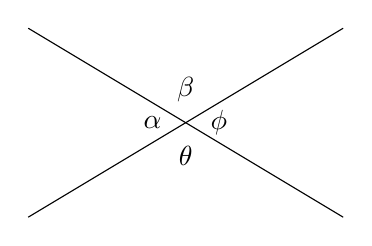
\begin{tikzpicture}
			\draw (-2,-1.2) coordinate (d) -- (2,1.2) coordinate (b);
			\draw (-2,1.2) coordinate (a) -- (2,-1.2) coordinate (c);
			\coordinate (o) at (0,0);
			\pic["$\theta$", angle radius=7mm] {angle=a--o--b};
			\pic["$\alpha$", angle radius=7mm] {angle=b--o--c};
			\pic["$\beta$", angle radius=7mm] {angle=c--o--d};
			\pic["$\phi$", angle radius=7mm] {angle=d--o--a};
		\end{tikzpicture}
	\end{center}

	\section*{Angles and Parallel Lines}
	\textbf{Parallel lines} are lines which go in the exact same direction.
	Two parallel lines are always the same distance apart.
	In the following figure, lines $l$ and $m$ are parallel; this is written as $l \parallel m$.
	Line $n$ is a \textbf{transversal}.
	Angles $\alpha$ and $\beta$ are called \textbf{alternate angles}, and alternate angles are always equal.
	Since $\gamma$ and $\alpha$ are vertical angles, they are equal, so $\alpha = \beta = \gamma$.
	The pair $\gamma$ and $\beta$ are called \textbf{corresponding angles}.
	Also, $\theta$ and $\beta$ together form a strait line and thus are supplementary.
	Since $\beta = \alpha$, we find that $\theta$ and $\alpha$ are also supplementary.
	The angles $\theta$ and $\alpha$ are sometimes called \textbf{same-side angles}.

	When you see vertical angles, corresponding angles, or alternate interior angles, it's often a good idea to mark them as equal on the diagram.
	This is done by drawing a small arc inside the angle.
	Any angle which has one such arc inside it is equal to all the other angles which have one arc inside.
	If we have another set of equal angles which are not equal to the first set, we draw two arcs inside the angles to distinguish between the two.
	Another notation is to draw one arc inside all angles and put tick marks on the arcs to indicate which angles are equal.
	In this notation angles with the same number of tick marks are equal.
	\begin{center}
		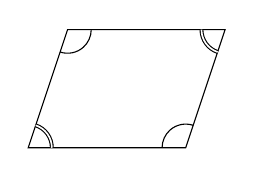
\begin{tikzpicture}
			\draw (0,0) coordinate (a) -- (0.5,1.5) coordinate (b)
				-- (2.5,1.5) coordinate (c) -- (2,0) coordinate (d) -- cycle
				pic[draw,angle radius=3mm] {angle=a--b--c}
				pic[draw,double,angle radius=3mm] {angle=b--c--d}
				pic[draw,angle radius=3mm] {angle=c--d--a}
				pic[draw,double,angle radius=3mm] {angle=d--a--b};
		\end{tikzpicture}
	\end{center}

	This figure shows that opposite angles in a parallelogram are equal.

	\section*{Circles}
	A circle is defined as the set of all points which are a fixed distance from a specific point called the center (point $O$ in the following figure).
	The fixed distance is called the radius.
	Here, the radius is $OA$, or the distance from point $O$ to $A$.
	A chord ($AC$) of a circle is a segment whose endpoints are both on the circle, and a diameter ($AB$) is a chord which passes through the center of the circle.
	(The words ``diameter'' and ``radius'' refer to both the segment and the length of the segment.)
	A tangent (line $l$) is a line which intersects the circle at exactly one point, and a secant (line $m$) is a line which passes through the circle, intersecting it in two places.
	Circles are often referred to by their centers, so we can call the circle in the figure circle $O$.
	A part of the curve is called an arc, and it is denoted by $\arc{AC}$ if $A$ and $C$ are the endpoints.
	\begin{center}
		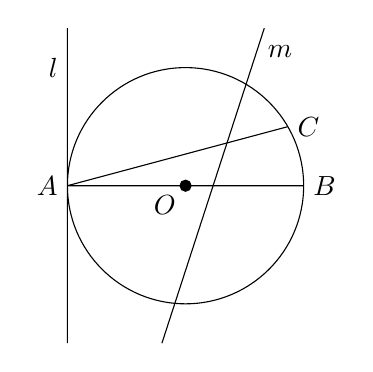
\begin{tikzpicture}
			\draw (0,0) coordinate (o) node[below left] {$O$} circle (1.5)
				(-1.5,-2) -- (-1.5,2)
				(-1.5,0) coordinate (a) node[left] {$A$} -- (1.5,0) coordinate (b) node[right] {$B$}
				(a) -- (30:1.5) coordinate (c) node[right] {$C$};
			\filldraw (o) circle (2pt);
			\node[left] at (-1.5,1.5) {$l$};
			\draw (-0.3, -2) -- (1, 2);
			\node at (1.2, 1.7) {$m$};
		\end{tikzpicture}
	\end{center}

	\section*{Angles Formed by Lines Intersecting a Circle}
	A \textbf{central angle} is an angle whose vertex is the center $O$ of a circle and whose sides are radii intersecting the circle in two distinct points $A$ and $B$.
	By definition, the measure of the central angle is equal to the measure of the arc which it subtends.
	\begin{center}
		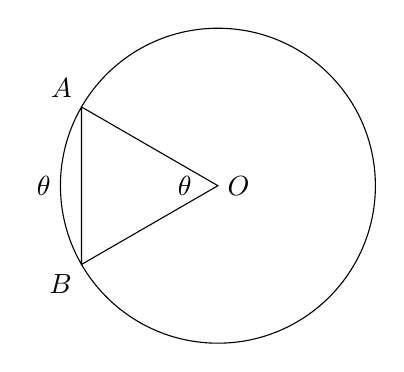
\begin{tikzpicture}
			\draw (0,0) coordinate (o) node[right] {$O$} circle (2)
				(o) -- (150:2) coordinate (a) node[above left] {$A$}
				-- (210:2) coordinate (b) node[below left] {$B$}
				-- cycle;
			\node[left] at (-2,0) {$\theta$};
			\pic["$\theta$",angle radius=7mm] {angle=a--o--b};
		\end{tikzpicture}
	\end{center}

	We will now look at angles formed by chords, tangents, and secants.

	An angle formed by two chords with a common endpoint is called an \textbf{inscribed angle}, and its measure is always half of the measure of the arc which it intercepts (or the central angle subtending the arc):
	\begin{center}
		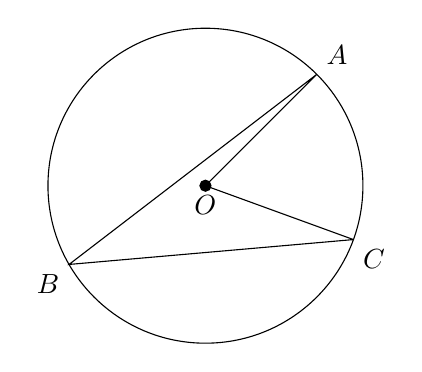
\begin{tikzpicture}
			\draw (0,0) coordinate (o) node[below] {$O$} circle (2)
				(45:2) coordinate (a) node[above right] {$A$}
				-- (210:2) coordinate (b) node[below left] {$B$}
				-- (-20:2) coordinate (c) node[below right] {$C$}
				(a) -- (o) -- (c);
			\filldraw (o) circle (2pt);
		\end{tikzpicture}
	\end{center}
	\[
		\angle ABC = \frac{\arc{AC}}{2} = \frac{\angle AOC}{2}
	\]
	This is known as the \textbf{inscribed angle theorem}.
	You can find a proof of it at \url{https://en.wikipedia.org/wiki/Inscribed_angle}.

	When we have two secants which intersect outside the circle, the measure of the angle formed by the two secants is half of the difference of the arcs intercepted by the secants:
	\begin{center}
		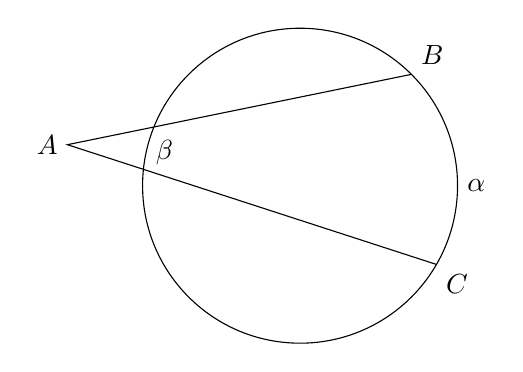
\begin{tikzpicture}
			\draw (0,0) circle (2)
				(45:2) coordinate (b) node[above right] {$B$}
				-- (170:3) coordinate (a) node[left] {$A$}
				-- (-30:2) coordinate (c) node[below right] {$C$};
			\node[right] at (0:2) {$\alpha$};
			\node[right] at (168:2) {$\beta$};
		\end{tikzpicture}
	\end{center}
	\[
		\angle BAC = \frac{\alpha - \beta}{2}
	\]
	This also works if one or both of the lines are tangents instead of secants.

	The angle formed by a tangent and a chord is half of the measure of the arc between the endpoints of the chord:
	\begin{center}
		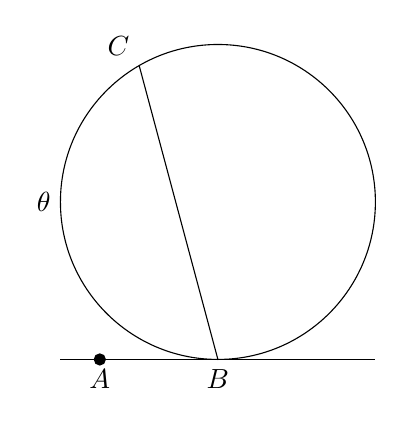
\begin{tikzpicture}
			\draw (0,0) circle (2)
				(0,-2) coordinate (b) node[below] {$B$}
				-- (120:2) coordinate (c) node[above left] {$C$};
			\draw (-2,-2) -- (2,-2);
			\filldraw (-1.5,-2) node[below] {$A$} circle (2pt);
			\node[left] at (-2,0) {$\theta$};
		\end{tikzpicture}
	\end{center}
	\[
		\angle ABC = \frac{\theta}{2}
	\]
	
	The angle formed by two chords is half of the sum of the intercepted arcs:
	\begin{center}
		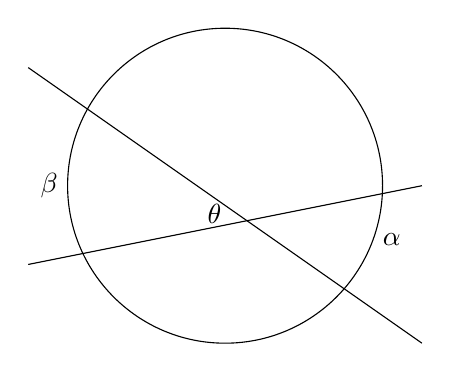
\begin{tikzpicture}
			\draw (0,0) circle (2);
			\draw[name path=A--B] (-2.5,-1) coordinate (A) -- (2.5,0) coordinate (B);
			\draw[name path=C--D] (-2.5,1.5) coordinate (C) -- (2.5,-2) coordinate (D);
			\path[name intersections={of=A--B and C--D,by=E}];
			\pic["$\theta$",angle radius=7mm] {angle=C--E--A};
			\node[left] at (-2,0) {$\beta$};
			\node[right] at (-20:2) {$\alpha$};
		\end{tikzpicture}
	\end{center}
	\[
		\theta = \frac{\alpha + \beta}{2}
	\]
\end{multicols}
\end{document}
